\documentclass[12pt,a4paper]{article}

% ---------- Basic packages ----------
\usepackage[margin=2.2cm]{geometry}
\usepackage[T1]{fontenc}
\usepackage[utf8]{inputenc}
\usepackage{lmodern}
\usepackage{microtype}
\usepackage{setspace}
\usepackage{parskip}
\usepackage{graphicx}
\usepackage{xcolor}
\usepackage{booktabs}
\usepackage{array}
\usepackage{longtable}
\usepackage{enumitem}
\usepackage{amsmath,amssymb}
\usepackage{hyperref}
\usepackage{fancyhdr}
\usepackage{titlesec}
\usepackage{caption}
\usepackage{float}
\usepackage{tabularx}
\usepackage{listings}
\usepackage{tikz}
\usepackage{pgfplots}
\usepackage[backend=biber,style=ieee]{biblatex}
\addbibresource{reference.bib}
\usetikzlibrary{arrows.meta,positioning,fit,shapes.geometric}
\pgfplotsset{compat=1.18}

% ---------- Hyperref setup ----------
\definecolor{DeepBlue}{HTML}{003A70}
\definecolor{ModelOrange}{HTML}{F28E2B}
\definecolor{ModelGreen}{HTML}{59A14F}
\definecolor{ModelRed}{HTML}{E15759}
\definecolor{PanelGray}{HTML}{F4F6F8}
\hypersetup{
    colorlinks=true,
    linkcolor=DeepBlue,
    citecolor=DeepBlue,
    urlcolor=DeepBlue,
    pdftitle={DTS406 Document Topic Classification Report},
    pdfauthor={Group AA}
}
\urlstyle{same}

% ---------- Line spacing ----------
\onehalfspacing
\renewcommand{\arraystretch}{1.15}

% ---------- Pseudocode listing style ----------
\definecolor{CodeGray}{HTML}{F2F2F2}
\definecolor{KeywordPurple}{HTML}{5B2C83}
\definecolor{CommentGreen}{HTML}{2E7D32}
\lstdefinestyle{pseudocode}{
    basicstyle=\ttfamily\footnotesize,
    backgroundcolor=\color{CodeGray},
    frame=single,
    framerule=0pt,
    xleftmargin=0.8em,
    xrightmargin=0.8em,
    framexleftmargin=0.8em,
    framexrightmargin=0.8em,
    breaklines=true,
    columns=fullflexible,
    keepspaces=true,
    showstringspaces=false,
    numbers=left,
    numberstyle=\scriptsize\color{gray},
    numbersep=0.6em,
    keywordstyle=\bfseries\color{KeywordPurple},
    commentstyle=\itshape\color{CommentGreen},
    morekeywords={FUNCTION,INPUT,OUTPUT,FOR,IF,ELSE,RETURN,TRAIN,FIT,TRANSFORM,PREDICT,UPDATE,POOL,CONVOLVE},
    morecomment=[l]{//},
    captionpos=b
}

% ---------- Section styling ----------
\titleformat{\section}{\large\bfseries}{\thesection.}{0.5em}{}
\titleformat{\subsection}{\normalsize\bfseries}{\thesubsection.}{0.5em}{}
\titleformat{\subsubsection}{\normalsize\itshape}{\thesubsubsection.}{0.5em}{}

% ---------- Header / footer ----------
\pagestyle{fancy}
\fancyhf{}
\lhead{DTS406 Document Topic Classification}
\rhead{Group AA}
\cfoot{\thepage}

% ---------- Report metadata ----------
\newcommand{\reporttitle}{Movie Genre Topic Classification with Traditional and Neural Models}
\newcommand{\groupid}{Group AA}
\newcommand{\modulename}{DTS406 Natural Language Processing}
\newcommand{\submissiondate}{19 May 2026}

\begin{document}

\begin{titlepage}
    \centering
    \vspace*{1.5cm}
    {\Large \textbf{Xi'an Jiaotong-Liverpool University}\par}
    \vspace{0.4cm}
    {\large School of AI and Advanced Computing\par}
    \vspace{2cm}
    {\huge \textbf{\reporttitle}\par}
    \vspace{1.2cm}
    {\Large Coursework Report\par}
    \vspace{2cm}
    \begin{tabular}{>{\bfseries}p{4cm}p{8.5cm}}
        Module: & \modulename \\
        Group: & \groupid \\
        Members: & Zijie Xue (2575576)\\
                 & Fengyuan Shu (2575904)\\
                 & Junyu Zhou (2575771)\\
        Submission Date: & \submissiondate \\
    \end{tabular}
    \vfill
    {\large Academic Year 2025--2026\par}
\end{titlepage}

\newpage
\tableofcontents
\newpage

\section{Individual Literature Reviews}
\subsection{Review 1: Zijie Xue --- User-Oriented Document Organisation}
I understand document topic classification as a way to reduce manual reading. Instead of opening every document, the system reads the text and places it under a useful topic label. Sebastiani treats this as a central task in automatic text categorisation \cite{sebastiani2002}. In real systems, this can support a news website that sorts articles into sections, a customer-service platform that sends tickets to different teams, or a movie website that groups films by genre.

The user value is clear, but the task is not clean. Movie genres overlap in daily use. A film can look like crime, thriller, and horror at the same time. Some labels also have many more examples than others, so a model may become more confident on large categories. The two datasets in this project add another problem: IMDb summaries sound more like short advertisements, while Wikipedia plots read like full story descriptions.

For this reason, I think simple and explainable baselines are still important. TF-IDF features can show which words are useful \cite{ramos2003}, while Linear SVM is a strong text-classification baseline \cite{joachims1998}. TextCNN is less transparent, but it can test whether neural models learn extra phrase patterns from embeddings \cite{kim2014cnn}. A good report should not only say which model wins, but also explain what kind of text each model is good at.

\subsection{Review 2: Fengyuan Shu --- Feature Representation and Algorithms}
From my view, the key question is how raw text becomes numbers. TF-IDF is a practical answer: it gives more weight to words that are important in one document but not common in all documents \cite{ramos2003}. This is why it is still used in tasks such as paper indexing, legal document search, and review classification. In movie plots, words like ``haunted'', ``spaceship'', or ``cowboy'' can become strong genre signals.

Feature design also creates risks. Sparse word features do not know that two different words may have related meanings. Long Wikipedia plots may include many names, places, and side events that are not useful for genre prediction. Compound labels make the situation harder because one source label may contain several possible target labels.

The four algorithms in this project give a useful technical comparison. Naive Bayes uses word statistics and is simple, but its independence assumption is strong. Linear SVM is usually strong for high-dimensional sparse text \cite{cortes1995svm,joachims1998}. TextCNN moves away from pure TF-IDF by using embeddings and convolution filters to detect short local patterns \cite{kim2014cnn}. TF-IDF MLP keeps the engineered TF-IDF input but adds a neural classifier, so it can learn non-linear combinations that a linear model cannot.

\subsection{Review 3: Junyu Zhou --- Model Behaviour and Evaluation}
My focus is evaluation. A topic classifier is useful only if its predictions are reliable across labels, not only good on average. This connects with the general goal of automatic text categorisation described by Sebastiani \cite{sebastiani2002}. Similar systems are used in email filtering, content moderation, and digital library organisation. In this project, every plot summary is treated as one document, and the target topic is the movie genre.

This is why accuracy alone is not enough. If a dataset has fewer examples for some genres, a model can obtain a fair accuracy while still missing the smaller classes. Macro precision, macro recall, and macro-F1 are more suitable because every genre contributes equally. They also make label confusion easier to discuss, such as action being mixed with adventure, or thriller being mixed with horror and crime.

The models should therefore be compared by both score and behaviour. Naive Bayes is easy to reproduce and gives a useful lower-complexity reference. Linear SVM often becomes the strongest traditional baseline when TF-IDF keywords are clear \cite{cortes1995svm,joachims1998}. TextCNN tests whether sequence-based neural learning helps when embeddings are trained from the project data \cite{kim2014cnn}. TF-IDF MLP is a different neural choice: it does not read word order directly, but it can combine word-level and character-level TF-IDF features in a non-linear way. This makes the final comparison more informative than simply trying four unrelated classifiers.

\section{Datasets and Preprocessing}
\subsection{Dataset Sources}
We use two public Kaggle datasets. The first is \textit{Genre Classification Dataset IMDb}, which contains short movie summaries and genre labels \cite{kaggle_imdb_genre}. The second is \textit{Wikipedia Movie Plots}, which contains longer plot descriptions from different countries and film industries \cite{kaggle_wiki_plots}. The two datasets are suitable because they are from different text scenarios: IMDb is short, emotional, and promotional, while Wikipedia is long, factual, and narrative.

\begin{table}[H]
\centering
\begin{tabular}{lrrrrrr}
\toprule
\textbf{Dataset} & \textbf{Samples} & \textbf{Labels} & \textbf{Vocab} & \textbf{Avg. length} & \textbf{Train} & \textbf{Test} \\
\midrule
IMDb & 10,000 & 10 & 39,013 & 55.56 & 8,000 & 2,000 \\
Wikipedia & 9,601 & 10 & 64,454 & 225.47 & 7,680 & 1,921 \\
\bottomrule
\end{tabular}
\caption{Processed dataset statistics. Document length is measured after TF-IDF-oriented token cleaning.}
\label{tab:dataset_stats}
\end{table}

\begin{figure}[H]
\centering
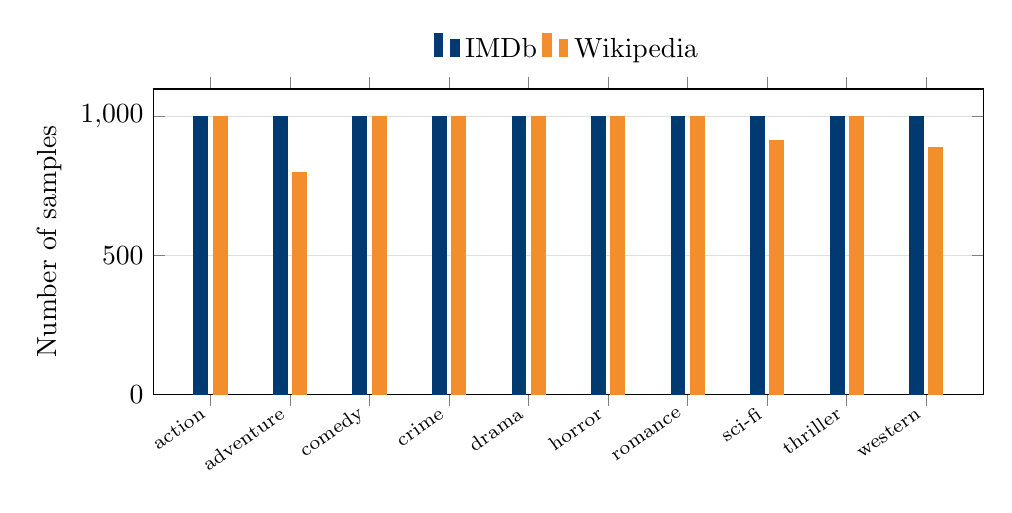
\begin{tikzpicture}
\begin{axis}[
    ybar,
    width=\linewidth,
    height=0.45\linewidth,
    ymin=0,
    ylabel={Number of samples},
    symbolic x coords={action,adventure,comedy,crime,drama,horror,romance,sci-fi,thriller,western},
    xtick=data,
    x tick label style={rotate=35, anchor=east, font=\scriptsize},
    ymajorgrids=true,
    grid style={draw=gray!25},
    bar width=5pt,
    enlarge x limits=0.08,
    legend style={at={(0.5,1.05)}, anchor=south, legend columns=2, draw=none}
]
\addplot+[fill=DeepBlue, draw=DeepBlue] coordinates {
    (action,1000) (adventure,1000) (comedy,1000) (crime,1000) (drama,1000) (horror,1000)
    (romance,1000) (sci-fi,1000) (thriller,1000) (western,1000)
};
\addplot+[fill=ModelOrange, draw=ModelOrange] coordinates {
    (action,1000) (adventure,799) (comedy,1000) (crime,1000) (drama,1000) (horror,1000)
    (romance,1000) (sci-fi,914) (thriller,1000) (western,888)
};
\legend{IMDb,Wikipedia}
\end{axis}
\end{tikzpicture}
\caption{Label distribution after mapping and balanced sampling. Some classes remain below 1000 because the source data did not contain enough usable samples.}
\label{fig:label_dist}
\end{figure}

\subsection{Cleaning and Label Mapping}
The original label spaces are different. IMDb has cleaner single labels, while Wikipedia contains labels such as \textit{romantic drama}, \textit{crime drama}, and many rare labels. We map both datasets into 10 shared labels, written here in the same priority order used for Wikipedia compound-genre mapping: horror, science\_fiction, thriller, adventure, action, crime, romance, comedy, western, and drama. IMDb \textit{sci-fi} is mapped to \textit{science\_fiction}. The priority order is needed because many Wikipedia labels contain more than one genre word. Earlier labels are checked first, so more distinctive or easily absorbed genres are kept before broader genres when a single final label must be chosen.

The cleaning steps are: removing empty texts, removing very short texts, removing Wikipedia citation marks, normalising spaces, lowercasing, tokenisation, stop-word removal, and lemmatisation. Two text fields are saved. \texttt{text\_clean\_tfidf} is used for TF-IDF and for final neural sequence input. \texttt{text\_clean\_dl} is kept as a lighter sequence-cleaned version, but the final report uses \texttt{text\_clean\_tfidf} because it reduces noise and improves model stability.

\begin{table}[H]
\centering
\begin{tabularx}{\linewidth}{p{0.26\linewidth}X}
\toprule
\textbf{Design choice} & \textbf{Reason} \\
\midrule
Use 10 shared labels & Keeps IMDb and Wikipedia comparable under the same classification task. \\
Drop unknown and unmapped labels & Avoids noisy labels that do not describe a clear movie genre. \\
Balance up to 1000 samples/class & Reduces the dominance of large classes such as drama and comedy. \\
Use stratified 80/20 split & Keeps similar label proportions in train and test sets. \\
Use title + cleaned text for neural models & Movie titles often contain useful genre signals, while cleaned text reduces noise. \\
\bottomrule
\end{tabularx}
\caption{Main preprocessing decisions and their motivation.}
\label{tab:preprocess_choices}
\end{table}

The processed datasets are close to balanced but still not perfect because some target genres do not have enough usable samples after cleaning. IMDb has 1000 examples for each shared label. Wikipedia still has 799 adventure samples, 914 science fiction samples, and 888 western samples. This is important for interpreting the results. Accuracy can look acceptable even when smaller classes are weak, so macro precision, macro recall, and macro-F1 are more informative.

\section{Algorithm Design and Implementation}
\subsection{System Pipeline}
The system is implemented in Python. Data cleaning scripts are under \texttt{utils/}. Training scripts are under \texttt{experiments/}. Traditional models use scikit-learn \cite{sklearn_docs}. Neural models use PyTorch \cite{pytorch_docs}. The same train-test split is used for all four models to make the comparison fair.

The implementation separates data preparation from experiments. The preprocessing script reads the raw IMDb text files and the Wikipedia CSV file, applies label mapping, writes two processed CSV files, and stores the split column. The analysis script then produces dataset statistics and word-frequency tables. This design makes later experiments reproducible: all models read the same processed files and do not create their own train-test splits.

\begin{figure}[H]
\centering
\resizebox{\linewidth}{!}{%
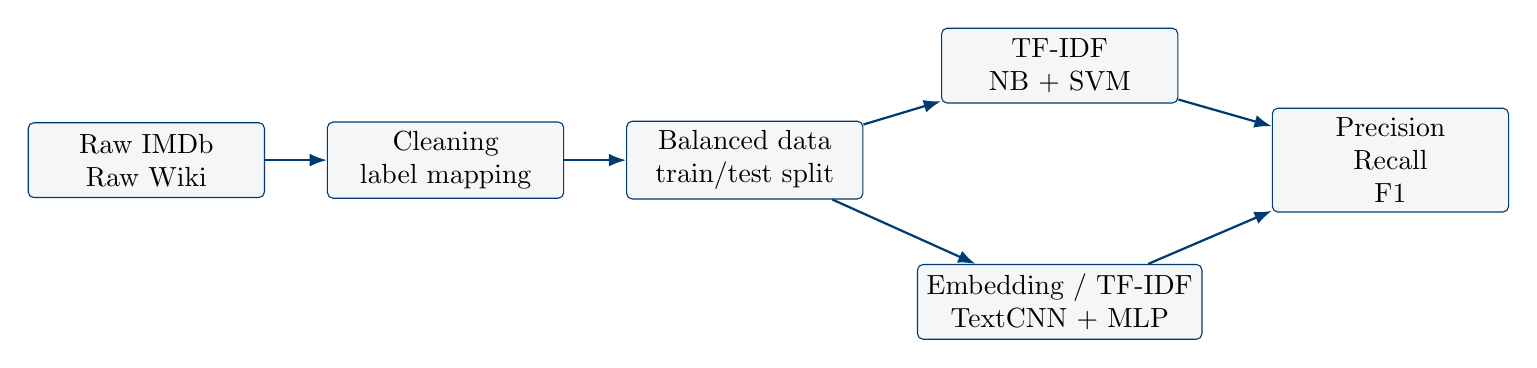
\begin{tikzpicture}[
    block/.style={draw=DeepBlue, rounded corners=2pt, fill=PanelGray, minimum width=3.0cm, minimum height=0.95cm, align=center},
    arrow/.style={-{Latex[length=2.2mm]}, thick, draw=DeepBlue}
]
\node[block] (raw) at (0,0) {Raw IMDb\\Raw Wiki};
\node[block] (clean) at (3.8,0) {Cleaning\\label mapping};
\node[block] (split) at (7.6,0) {Balanced data\\train/test split};
\node[block] (trad) at (11.6,1.2) {TF-IDF\\NB + SVM};
\node[block] (deep) at (11.6,-1.8) {Embedding / TF-IDF\\TextCNN + MLP};
\node[block] (eval) at (15.8,0) {Precision\\Recall\\F1};
\draw[arrow] (raw) -- (clean);
\draw[arrow] (clean) -- (split);
\draw[arrow] (split) -- (trad);
\draw[arrow] (split) -- (deep);
\draw[arrow] (trad) -- (eval);
\draw[arrow] (deep) -- (eval);
\end{tikzpicture}}
\caption{Overall experiment pipeline.}
\label{fig:pipeline}
\end{figure}

\subsection{Selected Models}
Naive Bayes is used as a fast probabilistic baseline. The text is first converted into TF-IDF features, and the classifier estimates which words are more likely under each genre. The pseudocode below shows the two key components: feature extraction and probability-based prediction.

\begin{lstlisting}[style=pseudocode,caption={Naive Bayes with TF-IDF.}]
FUNCTION TrainNaiveBayes(train_texts, train_labels):
    X_train = TFIDF(train_texts)
    model = MultinomialNB(alpha=0.5)
    FIT model on X_train and train_labels
    RETURN vectorizer, model

FUNCTION PredictNaiveBayes(vectorizer, model, test_texts):
    X_test = TRANSFORM test_texts with vectorizer
    RETURN PREDICT model on X_test
\end{lstlisting}

Linear SVM is the second traditional method. It uses TF-IDF unigram and bigram features, then learns a large-margin linear boundary. This is suitable for sparse text vectors because many genre clues appear as keywords or short phrases.

\begin{lstlisting}[style=pseudocode,caption={Linear SVM with TF-IDF.}]
FUNCTION TrainLinearSVM(train_texts, train_labels):
    X_train = TFIDF(train_texts, unigram_and_bigram=True)
    model = LinearSVM(class_weight="balanced")
    FIT model on X_train and train_labels
    RETURN vectorizer, model

FUNCTION PredictLinearSVM(vectorizer, model, test_texts):
    X_test = TRANSFORM test_texts with vectorizer
    RETURN PREDICT model on X_test
\end{lstlisting}

TextCNN is the first deep learning model. It reads token ids, looks up word embeddings, and applies convolution filters over local word windows. The max-pooling step keeps the strongest phrase signal for each filter. This follows the wider use of convolutional networks for text classification, including word-level CNNs and character-level CNNs \cite{kim2014cnn,zhang2015charcnn}.

\begin{lstlisting}[style=pseudocode,caption={TextCNN with word embeddings.}]
FUNCTION TrainTextCNN(train_tokens, train_labels):
    vocab = BUILD_VOCAB(train_tokens)
    input_ids = ENCODE_AND_PAD(train_tokens)
    FOR each epoch:
        embeddings = LOOKUP(input_ids)
        feature_maps = CONVOLVE embeddings with filter sizes 1,2,3,4,5
        pooled = MAX_POOL(feature_maps)
        logits = Linear(Dropout(pooled))
        UPDATE model using cross entropy loss
    RETURN model, vocab
\end{lstlisting}

TF-IDF MLP is the second deep learning model. Instead of reading token sequences, it uses word and character TF-IDF features as input to a multi-layer perceptron. This design keeps strong keyword features while allowing non-linear neural classification.

\begin{lstlisting}[style=pseudocode,caption={TF-IDF MLP neural classifier.}]
FUNCTION TrainTfidfMLP(train_texts, train_labels):
    X_train = WORD_AND_CHAR_TFIDF(train_texts)
    model = MLP(input_dim, hidden_dim=1024, output_dim=num_labels)
    FOR each epoch:
        logits = model(X_train)
        UPDATE model using cross entropy loss with label smoothing
    RETURN vectorizer, model
\end{lstlisting}

\subsection{Model Strengths and Weaknesses}
Naive Bayes is fast and simple, but it assumes words are independent. Linear SVM is strong for sparse TF-IDF features, but it does not learn semantic embeddings. TextCNN can learn local phrase patterns, but it needs enough training examples and good embeddings. TF-IDF MLP uses strong TF-IDF features and learns non-linear combinations, but it still does not directly understand word order.

The final four models intentionally cover different modelling ideas. Naive Bayes is a probabilistic baseline. Linear SVM is a strong margin-based traditional baseline. TextCNN is an embedding-based neural model that directly reads token sequences. TF-IDF MLP is a neural classifier over engineered text features. Therefore, the experiment does not only compare scores; it also compares whether keyword features, local phrase learning, or non-linear neural classification are more useful for movie genre prediction.

\begin{table}[H]
\centering
\begin{tabularx}{\linewidth}{p{0.18\linewidth}p{0.22\linewidth}p{0.27\linewidth}X}
\toprule
\textbf{Model} & \textbf{Input} & \textbf{Main advantage} & \textbf{Main weakness} \\
\midrule
Naive Bayes & TF-IDF words & Very fast and simple; good for keyword-heavy data. & Strong independence assumption; weak phrase understanding. \\
Linear SVM & TF-IDF words/bigrams & Strong in high-dimensional sparse text space. & Still surface-feature based; no learned semantics. \\
TextCNN & Token ids and embeddings & Learns local n-gram patterns from text. & Needs enough data and good embeddings; less stable on long noisy plots. \\
TF-IDF MLP & Word and character TF-IDF & Combines strong features with neural non-linearity. & Does not directly model word order or full story flow. \\
\bottomrule
\end{tabularx}
\caption{Advantages and limitations of the four selected algorithms.}
\label{tab:model_strengths}
\end{table}

\section{Experimental Results}
\subsection{Main Results}
We report macro precision, macro recall, and macro-F1 because the dataset is not perfectly balanced. Macro scores treat each class equally, so weak performance on smaller classes is visible.

\begin{table}[H]
\centering
\begin{tabular}{llrrrr}
\toprule
\textbf{Dataset} & \textbf{Model} & \textbf{Accuracy} & \textbf{Macro P} & \textbf{Macro R} & \textbf{Macro F1} \\
\midrule
IMDb & Naive Bayes & \textbf{0.5935} & 0.5952 & \textbf{0.5935} & 0.5864 \\
IMDb & Linear SVM & 0.5925 & 0.5870 & 0.5925 & \textbf{0.5878} \\
IMDb & TextCNN & 0.5410 & 0.5437 & 0.5410 & 0.5377 \\
IMDb & TF-IDF MLP & 0.5885 & \textbf{0.5956} & 0.5885 & 0.5849 \\
\midrule
Wikipedia & Naive Bayes & 0.5757 & 0.5832 & 0.5776 & 0.5629 \\
Wikipedia & Linear SVM & 0.5836 & 0.5818 & 0.5889 & 0.5834 \\
Wikipedia & TextCNN & 0.5450 & 0.5703 & 0.5512 & 0.5491 \\
Wikipedia & TF-IDF MLP & \textbf{0.5872} & \textbf{0.5903} & \textbf{0.5930} & \textbf{0.5895} \\
\bottomrule
\end{tabular}
\caption{Four-model classification results on the two datasets. P, R, and F1 are macro-averaged.}
\label{tab:main_results}
\end{table}

\begin{figure}[H]
\centering
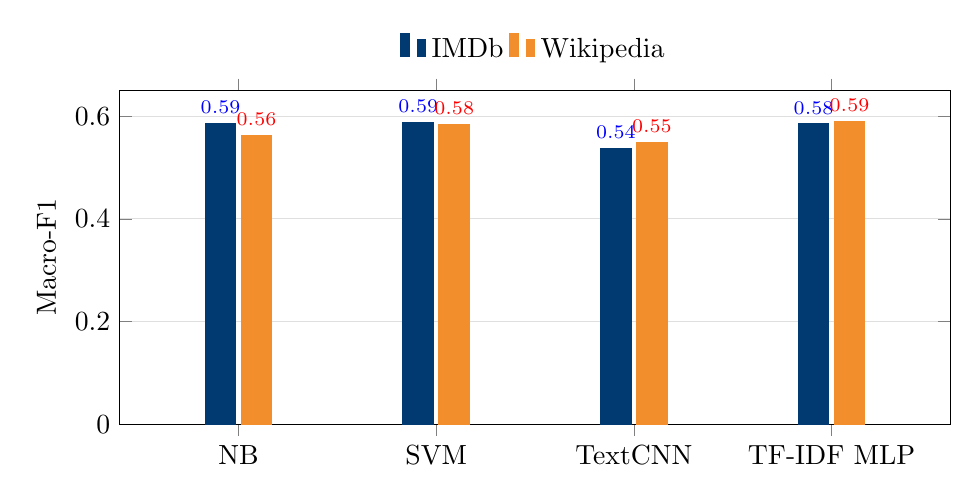
\begin{tikzpicture}
\begin{axis}[
    ybar,
    width=\linewidth,
    height=0.48\linewidth,
    ymin=0,
    ymax=0.65,
    ylabel={Macro-F1},
    symbolic x coords={NB,SVM,TextCNN,TF-IDF MLP},
    xtick=data,
    ymajorgrids=true,
    grid style={draw=gray!25},
    bar width=11pt,
    enlarge x limits=0.2,
    legend style={at={(0.5,1.05)}, anchor=south, legend columns=2, draw=none},
    nodes near coords,
    nodes near coords style={font=\scriptsize},
]
\addplot+[fill=DeepBlue, draw=DeepBlue] coordinates {
    (NB,0.5864) (SVM,0.5878) (TextCNN,0.5377) (TF-IDF MLP,0.5849)
};
\addplot+[fill=ModelOrange, draw=ModelOrange] coordinates {
    (NB,0.5629) (SVM,0.5834) (TextCNN,0.5491) (TF-IDF MLP,0.5895)
};
\legend{IMDb,Wikipedia}
\end{axis}
\end{tikzpicture}
\caption{Macro-F1 comparison of the four models.}
\label{fig:f1_comparison}
\end{figure}

\begin{figure}[H]
\centering
\begin{minipage}{0.48\linewidth}
\centering

\includegraphics[width=\linewidth]{figures/training_curves/imdb_training_loss.png}
\end{minipage}
\hfill
\begin{minipage}{0.48\linewidth}
\centering
\includegraphics[width=\linewidth]{figures/training_curves/wiki_training_loss.png}
\end{minipage}
\caption{Training loss curves for the two deep learning models. The shorter TF-IDF MLP curves reflect early stopping.}
\label{fig:training_loss}
\end{figure}

\begin{figure}[H]
\centering
\begin{minipage}{0.48\linewidth}
\centering

\includegraphics[width=\linewidth]{figures/training_curves/imdb_validation_macro_f1.png}
\end{minipage}
\hfill
\begin{minipage}{0.48\linewidth}
\centering

\includegraphics[width=\linewidth]{figures/training_curves/wiki_validation_macro_f1.png}
\end{minipage}
\caption{Validation macro-F1 curves for TextCNN and TF-IDF MLP. The curves show why early stopping can select an earlier epoch instead of the final epoch.}
\label{fig:val_f1}
\end{figure}

\begin{figure}[H]
\centering
\begin{minipage}{0.48\linewidth}
\centering

\includegraphics[width=\linewidth]{figures/confusion_matrices/imdb_linear_svm_confusion_matrix.png}
\end{minipage}
\hfill
\begin{minipage}{0.48\linewidth}
\centering
\includegraphics[width=\linewidth]{figures/confusion_matrices/wiki_tfidf_mlp_confusion_matrix.png}
\end{minipage}
\caption{Representative confusion matrices: Linear SVM on IMDb and TF-IDF MLP on Wikipedia.}
\label{fig:confusion_examples}
\end{figure}

\subsection{Analysis}
On IMDb, Linear SVM gives the best macro-F1 by a very small margin, while Naive Bayes gives the highest accuracy and TF-IDF MLP gives the highest macro precision. This dataset contains short summaries with strong genre words, so TF-IDF features are very useful for all three TF-IDF-based models. The differences among Naive Bayes, Linear SVM, and TF-IDF MLP are small, which suggests that the cleaned IMDb task is mainly driven by clear keyword evidence.

On Wikipedia, TF-IDF MLP is the best model. Wikipedia plots are much longer, and many documents contain mixed events, names, and subplots. TF-IDF still works well because it can focus on important words across long documents. The MLP slightly improves over Linear SVM because it can learn non-linear combinations of word and character TF-IDF features. The long Wikipedia plots also contain many character names and detailed events that are not directly useful for genre classification, which still limits the improvement.

TextCNN performs lower than the TF-IDF-based models on both datasets. This does not mean CNN is useless for text classification. It means that in this project, embeddings are trained from scratch and the data size is medium. Without pretrained word vectors, the model has to learn both word meanings and classification boundaries from the same limited data. Also, Wikipedia is still not perfectly balanced: adventure, science fiction, and western are below 1000 samples. This hurts macro-F1 because minority labels contribute equally to the final score.

The training curves in Figures~\ref{fig:training_loss} and~\ref{fig:val_f1} also explain the neural results. TextCNN keeps reducing training loss for more epochs, but the validation macro-F1 moves up and down. This means lower training loss does not always mean better generalisation. TF-IDF MLP reaches its best validation score early, so early stopping prevents it from fitting too strongly to the training split.

Naive Bayes is competitive on IMDb but weaker on Wikipedia. Its simple word-count assumption works better for short promotional summaries than for long plots. Linear SVM is more stable because it handles many sparse features and uses a margin-based decision boundary. The confusion matrices in Figure~\ref{fig:confusion_examples} show that many errors happen between semantically close genres. For example, action and adventure can overlap, while thriller, horror, and crime can share similar plot words.

Precision, recall, and F1 tell slightly different stories. Precision measures how many predicted items of a class are correct. Recall measures how many true items of a class are found. F1 balances the two. In this task, macro recall is important because a model can get good accuracy by predicting common classes but still miss smaller genres. For example, adventure can be confused with action because many films contain both action scenes and travel or quest elements. This is why the report focuses on macro-F1 rather than accuracy alone.

\subsection{Error Sources}
There are four main sources of error. First, genre labels are not always mutually exclusive. A film labelled as thriller may also look like horror or crime from its plot. Second, the Wikipedia genre field is noisy and often compound. Although we use a priority mapping rule, a single-label mapping cannot fully represent multi-genre films. Third, the two datasets have different writing styles. IMDb text is closer to marketing language, while Wikipedia text includes the whole story. Fourth, some genres have fewer samples even after balancing. These factors explain why no model achieves very high scores.

The results also show a useful lesson about deep learning. A more complex input pipeline is not always better. TextCNN tries to learn embeddings and phrase filters from the same medium-sized training data, while TF-IDF MLP starts from a stronger text representation that already highlights important words. This makes TF-IDF MLP more stable for this coursework setting. For future work, pretrained embeddings or larger labelled movie datasets may improve the embedding-based model.

\subsection{Reproducibility}
All output tables are generated from project files. The cleaned datasets are saved in \texttt{data/processed/}. Dataset statistics are saved in \texttt{outputs/tables/}. Model reports and prediction files are saved in \texttt{outputs/results/}. The final comparison table is saved as:
\texttt{outputs/results/model\_comparison.csv}

The generated figures are saved in \texttt{outputs/figures/}. The deep learning environment uses PyTorch CUDA 12.6 on the local GPU. Since the scripts fix the random seed, the results should be close when rerun under the same software versions, although small GPU numerical differences may still occur.

\section{Conclusion}
This project implements a complete document topic classification system on two movie text datasets. The results show that dataset style matters. Short IMDb summaries and long Wikipedia plots behave differently. Traditional TF-IDF models remain very strong, especially Linear SVM. Neural models are still useful: TextCNN provides a standard deep text classification baseline, and TF-IDF MLP shows that combining feature engineering with neural classification can be effective. However, deep learning is not automatically better. For medium-sized datasets with uneven labels and strong keyword signals, simple traditional methods can still be the most reliable choice.

\newpage
\printbibliography

\end{document}
